% chktex-file 2% chktex-file 29
% chktex-file 13
\documentclass{report}
\usepackage{setspace}
\usepackage[a4paper, total={7in, 10in}]{geometry}
\usepackage[fleqn]{amsmath}
\usepackage{empheq}
\usepackage{amssymb}
\usepackage{amsthm}
\usepackage{gensymb}
\usepackage[fleqn]{cases}
\usepackage{multicol}
\usepackage{color}
\usepackage{stix}
\usepackage{chngcntr}
\usepackage{tikz}
\usepackage{enumitem}
\usepackage{pgfplots}
\usepackage{etoolbox}
\usepackage{tikz-3dplot}
\usepackage{svg}
\usetikzlibrary{calc,matrix,arrows}
\usetikzlibrary{decorations.pathmorphing,patterns, calligraphy}

\tikzset{
    right angle quadrant/.code={
            \pgfmathsetmacro\quadranta{{1,1,-1,-1}[#1-1]}     % Arrays for selecting quadrant
            \pgfmathsetmacro\quadrantb{{1,-1,-1,1}[#1-1]}},
    right angle quadrant=1, % Make sure it is set, even if not called explicitly
    right angle length/.code={\def\rightanglelength{#1}},   % Length of symbol
    right angle length=2ex, % Make sure it is set...
    right angle symbol/.style n args={3}{
            insert path={
                    let \p0 = ($(#1)!(#3)!(#2)$) in     % Intersection
                    let \p1 = ($(\p0)!\quadranta*\rightanglelength!(#3)$), % Point on base line
                    \p2 = ($(\p0)!\quadrantb*\rightanglelength!(#2)$) in % Point on perpendicular line
                    let \p3 = ($(\p1)+(\p2)-(\p0)$) in  % Corner point of symbol
                    (\p1) -- (\p3) -- (\p2)
                }
        }
}

\tikzset{
    annotated cuboid/.pic={
            \tikzset{%
                every edge quotes/.append style={midway, auto},
                /cuboid/.cd,
                #1
            }
            \draw [every edge/.append style={pic actions, densely dashed, opacity=.5}, pic actions]
            (0,0,0) coordinate (o) -- ++(-\cubescale*\cubex,0,0) coordinate (a) -- ++(0,-\cubescale*\cubey,0) coordinate (b) edge coordinate [pos=1] (g) ++(0,0,-\cubescale*\cubez)  -- ++(\cubescale*\cubex,0,0) coordinate (c) -- cycle
            (o) -- ++(0,0,-\cubescale*\cubez) coordinate (d) -- ++(0,-\cubescale*\cubey,0) coordinate (e) edge (g) -- (c) -- cycle
            (o) -- (a) -- ++(0,0,-\cubescale*\cubez) coordinate (f) edge (g) -- (d) -- cycle;
            \path [every edge/.append style={pic actions, |-|}]
            (b) +(0,-5pt) coordinate (b1) edge ["\cubex \cubeunits"'] (b1 -| c)
            (b) +(-5pt,0) coordinate (b2) edge ["\cubey \cubeunits"] (b2 |- a)
            (c) +(3.5pt,-3.5pt) coordinate (c2) edge ["\cubez \cubeunits"'] ([xshift=3.5pt,yshift=-3.5pt]e)
            ;
        },
    /cuboid/.search also={/tikz},
    /cuboid/.cd,
    width/.store in=\cubex,
    height/.store in=\cubey,
    depth/.store in=\cubez,
    units/.store in=\cubeunits,
    scale/.store in=\cubescale,
    width=10,
    height=10,
    depth=10,
    units=cm,
    scale=.1,
}

\counterwithout{equation}{chapter}
\setlength{\columnseprule}{1pt}
\setlength{\columnsep}{24pt}
\setcounter{chapter}{14}
\hfuzz=100pt

\newcommand{\pgfplotsdrawaxis}{\pgfplots@draw@axis}
\makeatother
\pgfplotsset{only axis on top/.style={axis on top=false, after end axis/.code={
                    \pgfplotsset{axis line style=opaque, ticklabel style=opaque, tick style={thick,opaque},
                        grid=none}\pgfplotsdrawaxis}}}

\newtheorem{theorem}{Theorem}

\begin{document}

\newcommand{\planelineinter}[5]% a, b, c, p as {a_x,a_y,a_z}, coordinate name
{   \foreach \a [count=\k] in {#1}
        { \ifthenelse{\k=1}{\xdef\tempxa{\a}}
            \ifthenelse{\k=2}{\xdef\tempya{\a}}
            \ifthenelse{\k=3}{\xdef\tempza{\a}}
        }
    \foreach \b [count=\k] in {#2}
        { \ifthenelse{\k=1}{\xdef\tempxb{\b}}
            \ifthenelse{\k=2}{\xdef\tempyb{\b}}
            \ifthenelse{\k=3}{\xdef\tempzb{\b}}
        }
    \foreach \c [count=\k] in {#3}
        { \ifthenelse{\k=1}{\xdef\tempxc{\c}}
            \ifthenelse{\k=2}{\xdef\tempyc{\c}}
            \ifthenelse{\k=3}{\xdef\tempzc{\c}}
        }
    \foreach \p [count=\k] in {#4}
        { \ifthenelse{\k=1}{\xdef\tempxp{\p}}
            \ifthenelse{\k=2}{\xdef\tempyp{\p}}
            \ifthenelse{\k=3}{\xdef\tempzp{\p}}
        }
    \pgfmathsetmacro{\abx}{\tempxb-\tempxa}
    \pgfmathsetmacro{\aby}{\tempyb-\tempya}
    \pgfmathsetmacro{\abz}{\tempzb-\tempza}
    \pgfmathsetmacro{\acx}{\tempxc-\tempxa}
    \pgfmathsetmacro{\acy}{\tempyc-\tempya}
    \pgfmathsetmacro{\acz}{\tempzc-\tempza}
    \pgfmathsetmacro{\nx}{\aby*\acz-\abz*\acy}
    \pgfmathsetmacro{\ny}{\abz*\acx-\abx*\acz}
    \pgfmathsetmacro{\nz}{\abx*\acy-\aby*\acx}
    \pgfmathsetmacro{\d}{(\nx+\ny+\nz)/(\nx*\tempxp+\ny*\tempyp+\nz*\tempzp)}
    \path (0,0,0) -- (#4) coordinate[pos=\d] (#5);
}

% golden ratio and inverse golden ratio
\pgfmathsetmacro{\gr}{(1+sqrt(5))/2}
\pgfmathsetmacro{\igr}{2/(1+sqrt(5))}

%choose axis angles
\newcommand{\xangle}{0}
\newcommand{\yangle}{90}
\newcommand{\zangle}{225}

%choose axis lengths
\newcommand{\xlength}{1}
\newcommand{\ylength}{1}
\newcommand{\zlength}{0.5}

\pgfmathsetmacro{\xx}{\xlength*cos(\xangle)}
\pgfmathsetmacro{\xy}{\xlength*sin(\xangle)}
\pgfmathsetmacro{\yx}{\ylength*cos(\yangle)}
\pgfmathsetmacro{\yy}{\ylength*sin(\yangle)}
\pgfmathsetmacro{\zx}{\zlength*cos(\zangle)}
\pgfmathsetmacro{\zy}{\zlength*sin(\zangle)}

\newcommand{\sol}[1]{

    \noindent \textbf{Sol.}
}
\newcommand{\prooff}[1]{

    \noindent \textbf{Proof.}
}
\newcommand\m[1]{\begin{pmatrix}#1\end{pmatrix}}
\newcommand\vm[1]{\begin{vmatrix}#1\end{vmatrix}}
\newenvironment{amatrix}[1]{%
    \left(\begin{array}{@{}*{#1}{c}|c@{}}
        }{%
    \end{array}\right)
}
\newenvironment{cequation}{
    \makeatletter
    \setbool{@fleqn}{false}
    \makeatother
    \begin{equation*}
        }{\end{equation*}}

\begin{titlepage}
    \raggedleft{}
    \rule{1pt}{\textheight}
    \hspace{0.02\textwidth}
    \parbox[b]{0.75\textwidth}{

    {\Huge\bfseries Solution Book of \\[0.5\baselineskip] Mathematic}\\[2\baselineskip]
    {\large\textit{Ssnior 2 Part I}}\\[4\baselineskip]
    {\Large\textsc{MELVIN CHIA}}

    \vspace{0.5\textheight}

    {\noindent Written on 9 October 2022}\\[\baselineskip]
    }

\end{titlepage}

\doublespacing{}
\tableofcontents
\singlespacing{}
\newpage

\begin{multicols}{2}

    \chapter{Solid Geometry, Longitude and Latitude}

    \section{Solid Geometry}

    \subsection*{Polyhedron}

    A polyhedron is a solid bounded by a finite amount of flat polygon, and each
    side of the polygons must be the common edge of two polygons. Polyhedron can be
    classified into tetrahedron, pentahedron, hexahedron, etc. based on the number
    of flat surfaces, aka the \emph{faces} of the polyhedron. The common side of
    two faces of a polyhedron is called an edge, and the common vertex of three
    edges is called an \emph{apex}.

    Besides, the angles formed by the faces intersecting at the same vertex are
    called polyhedral angles or solid angles. The line segment connecting two
    apexes at different faces is called a \emph{diagonal}.

    \begin{center}
        \tdplotsetmaincoords{70}{70}
        \begin{tikzpicture}[scale=0.6,tdplot_main_coords,declare function={d=6;}]
            \path (0,0,0)       coordinate (A)
            (d/2,d/2,0)     coordinate (H)
            (d,0,0)        coordinate (C)
            (d/2,{d*sqrt(3)/2},0)    coordinate (B)
            (d/2,d/2,{d/sqrt(2)}) coordinate (D)
            ($ (A)!0.5!(C) $) coordinate (M);
            \foreach \p/\g in {A/-90,B/-90,C/-90,D/90}
            \path (\p)+(\g:3mm);
            \draw (D) -- (A) (D) -- (B) (D) -- (C) (A) -- (C) -- (B);
            \draw [dashed] (A) -- (B);
            \node at (C) [below=10pt] {Tetrahedron};
        \end{tikzpicture}
        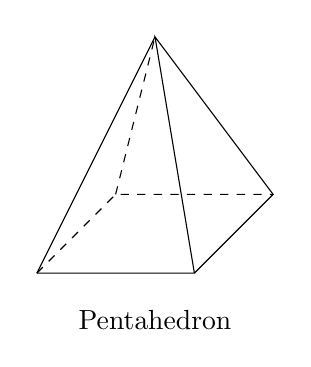
\begin{tikzpicture}
            \tikzstyle{point}=[circle,thick,draw=black,fill=black,inner sep=0pt,minimum width=4pt,minimum height=4pt]
            \node (a) at (0,0) {};
            \node (b) at (2,0) {};
            \node (c) at (3,1) {};
            \node (d) at (1,1) {};
            \node (e) at (1.5,3) {};
            \draw (a.center) -- (b.center) -- (c.center) -- (e.center) -- (b.center);
            \draw (a.center) -- (e.center);
            \draw[dashed] (a.center) -- (d.center) -- (c.center);
            \draw[dashed] (d.center) -- (e.center);
            \node at (1.5,0) [below=10pt] {Pentahedron};
        \end{tikzpicture}
    \end{center}
    \begin{center}
        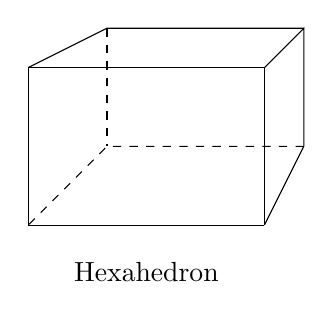
\begin{tikzpicture}
            \draw (0,0)--(3,0);
            \draw (3,0)--(3.5,1);
            \draw[dashed] (3.5,1)--(1,1)--(0,0);
            \draw (0,0)--(0,2)--(3,2)--(3,0);
            \draw (0,2)--(1,2.5)--(3.5,2.5);
            \draw[] (3,2)--(3.5,2.5)--(3.5,1);
            \draw[dashed] (1,2.5)--(1,1);
            \node at (1.5,0) [below=10pt] {Hexahedron};
        \end{tikzpicture}
    \end{center}

    \subsection*{Regular Polyhedron}

    A regular polyhedron is a polyhedron with all faces being regular polygons, and
    all polyhedral angles being equal. The regular polyhedron can be classified
    into 5 types: tetrahedron, octahedron, cube, icosahedron and dodecahedron.

    \begin{center}
        \tdplotsetmaincoords{70}{100}
        \begin{tikzpicture}[scale=0.7,line join=round,tdplot_main_coords,declare function={a=5;}]
            \begin{scope}[canvas is xy plane at z=0,transform shape]
                \path foreach \X [count=\Y] in {A,B,C}
                    {(\Y*120:{a/(2*cos(30))}) coordinate(\X)};
            \end{scope}
            \path (0,0,{a*cos(30)}) coordinate (D);
            \draw [dashed] (A) -- (D) -- (B) -- (A);
            \draw (B) -- (D) -- (C) -- (B);
            \draw (C) -- (D) -- (A) -- (C);
            \node at (0,0,0) [below=30pt] {Regular Tetrahedron};
        \end{tikzpicture}
        \hspace*{1cm}
        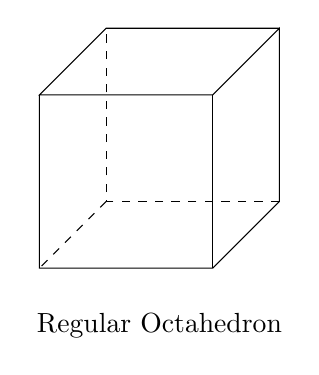
\begin{tikzpicture}[scale=1.1]
            \draw (2,2,0)--(0,2,0)--(0,2,2)--(2,2,2)--(2,2,0)--(2,0,0)--(2,0,2)--(0,0,2)--(0,2,2);
            \draw (2,2,2)--(2,0,2);
            \draw[dashed](2,0,0)--(0,0,0)--(0,2,0);
            \draw[dashed](0,0,0)--(0,0,2);
            \node at (1,1,1) [below=56pt] {Regular Octahedron};
        \end{tikzpicture}
    \end{center}

    \begin{center}
        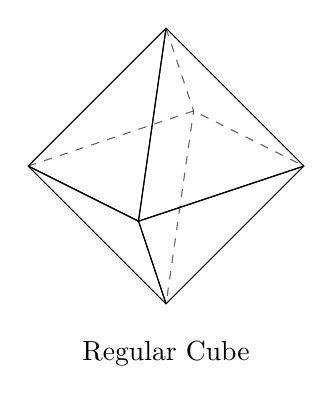
\begin{tikzpicture}[scale=3.5]

            \coordinate (A1) at (0,0);
            \coordinate (A2) at (0.6,0.2);
            \coordinate (A3) at (1,0);
            \coordinate (A4) at (0.4,-0.2);
            \coordinate (B1) at (0.5,0.5);
            \coordinate (B2) at (0.5,-0.5);

            \begin{scope}[dashed,opacity=0.6]
                \draw (A1) -- (A2) -- (A3);
                \draw (B1) -- (A2) -- (B2);
            \end{scope}
            \draw (A1) -- (A4) -- (B1);
            \draw (A1) -- (A4) -- (B2);
            \draw (A3) -- (A4) -- (B1);
            \draw (A3) -- (A4) -- (B2);
            \draw (B1) -- (A1) -- (B2) -- (A3) --cycle;
            \node at (0.5,-0.5) [below=10pt] {Regular Cube};
        \end{tikzpicture}
        \hspace*{1cm}
        \begin{tikzpicture}[scale=1]
            [   x={(\xx cm,\xy cm)},
                y={(\yx cm,\yy cm)},
                z={(\zx cm,\zy cm)},
                scale=2,
            ]

            % vertices of inscribed cube
            \coordinate (pd1) at (-1,-1,-1);
            \coordinate (pd2) at (-1,-1,1);
            \coordinate (pd3) at (-1,1,-1);
            \coordinate (pd4) at (-1,1,1);
            \coordinate (pd5) at (1,-1,-1);
            \coordinate (pd6) at (1,-1,1);
            \coordinate (pd7) at (1,1,-1);
            \coordinate (pd8) at (1,1,1);
            % "front/back" "outside of cube" points
            \coordinate (pd9) at (0,-\igr,-\gr);
            \coordinate (pd10) at (0,-\igr,\gr);
            \coordinate (pd11) at (0,\igr,-\gr);
            \coordinate (pd12) at (0,\igr,\gr);
            % "top/bottom" "outside of cube" points
            \coordinate (pd13) at (-\igr,-\gr,0);
            \coordinate (pd14) at (-\igr,\gr,0);
            \coordinate (pd15) at (\igr,-\gr,0);
            \coordinate (pd16) at (\igr,\gr,0);
            % "left/right" "outside of cube" points
            \coordinate (pd17) at (-\gr,0,-\igr);
            \coordinate (pd18) at (-\gr,0,\igr);
            \coordinate (pd19) at (\gr,0,-\igr);
            \coordinate (pd20) at (\gr,0,\igr);

            % edges on "back"    face of inscribes cube; red
            \draw[dashed] (pd9) -- (pd11);
            \draw[dashed] (pd11) -- (pd3);
            \draw[dashed] (pd11) -- (pd7);
            \draw[dashed] (pd9) -- (pd1);
            \draw[dashed] (pd9) -- (pd5);
            % edges on "top"     face of inscribes cube
            \draw[] (pd14) -- (pd16);
            \draw[] (pd16) -- (pd8);
            \draw[] (pd16) -- (pd7);
            \draw[dashed] (pd14) -- (pd3);
            \draw[] (pd14) -- (pd4);
            % edges on "left"    face of inscribes cube
            \draw[dashed] (pd17) -- (pd18);
            \draw[dashed] (pd17) -- (pd3);
            \draw[dashed] (pd17) -- (pd1);
            \draw[] (pd18) -- (pd2);
            \draw[] (pd18) -- (pd4);
            % edges on "bottom"  face of inscribes cube
            \draw[] (pd13) -- (pd15);
            \draw[dashed] (pd13) -- (pd1);
            \draw[] (pd13) -- (pd2);
            \draw[] (pd15) -- (pd5);
            \draw[] (pd15) -- (pd6);
            % edges on "front"   face of inscribes cube
            \draw[] (pd10) -- (pd12);
            \draw[] (pd12) -- (pd4);
            \draw[] (pd12) -- (pd8);
            \draw[] (pd10) -- (pd2);
            \draw[] (pd10) -- (pd6);
            % edges on "right"   face of inscribes cube 
            \draw[] (pd20) -- (pd19);
            \draw[] (pd19) -- (pd7);
            \draw[] (pd19) -- (pd5);
            \draw[] (pd20) -- (pd8);
            \draw[] (pd20) -- (pd6);

            \node at (0,-2.4,0) {Regular Dodecahedron};
        \end{tikzpicture}
    \end{center}
    \begin{center}
        \def \phi {1.617}
        \begin{tikzpicture}[
                x={(-0.86in, -0.5in)}, y = {(0.86in, -0.5in)}, z = {(0, 1in)},
                rotate = 22,
                scale = 0.2,
                foreground/.style = {  },
                background/.style = { dashed }
            ]
            \coordinate (9) at (0, -\phi*\phi,  \phi);
            \coordinate (8) at (0,  \phi*\phi,  \phi);
            \coordinate (12) at (0,  \phi*\phi, -\phi);
            \coordinate (5) at (0, -\phi*\phi, -\phi);
            \coordinate (7) at ( \phi, 0,  \phi*\phi);
            \coordinate (3) at (-\phi, 0,  \phi*\phi);
            \coordinate (6) at (-\phi, 0, -\phi*\phi);
            \coordinate (4) at ( \phi, 0, -\phi*\phi);
            \coordinate (2) at ( \phi*\phi,  \phi, 0);
            \coordinate (10) at (-\phi*\phi,  \phi, 0);
            \coordinate (1) at (-\phi*\phi, -\phi, 0);
            \coordinate (11) at ( \phi*\phi, -\phi, 0);

            \draw[foreground] (10) -- (3) -- (8) -- (10) -- (12) -- (8);
            \draw[foreground] (4) -- (12) -- (2) -- (4) -- (11) -- (2);
            \draw[foreground] (9) -- (3) -- (7) -- (9) -- (11) -- (7);
            \draw[foreground] (7) -- (8) -- (2) -- cycle;
            \draw[background] (12) -- (6) -- (10) -- (1) -- (6) -- (5) -- (1)
            -- (9) -- (5) -- (11);
            \draw[background] (5) -- (4) -- (6);
            \draw[background] (3) -- (1);

            \node at (6,3.8,0) {Regular Icosahedron};
        \end{tikzpicture}
    \end{center}

\end{multicols}
\end{document}